\section{Balancing}
\label{section:node-level:balancing}

\begin{hypothesis}
 The code is split up into a sufficiently large chunk of concurrent sections, but these sections are of massively different size.
 It is this imbalance that harms the performance.
\end{hypothesis}


If work is imbalanced, some cores will idle at one point.
If we do not exploit all cores all the time, we cannot expect to squeeze out all of the performance of the node.


\subsection{Model}

\begin{performancemetric}
  In line with all other metrics, we consider a code phase or loop reasonably balanced, if it is able to exploit around 80\% of the available compute resources at any point in time.
  If we underrun this threshold, the code is not super balanced.
\end{performancemetric}



\subsection{Data collection}

Most profilers have quite an extensive support to identify ill-balancing.
After all, this is the most obvious, ultimative, original sin of non-scaling.

\begin{instructions}{\vtune}
 The hotspot and threading analysis of \vtune~both offer you a bottom-up view, where imbalances are clearly visible:
 
 \begin{center}
   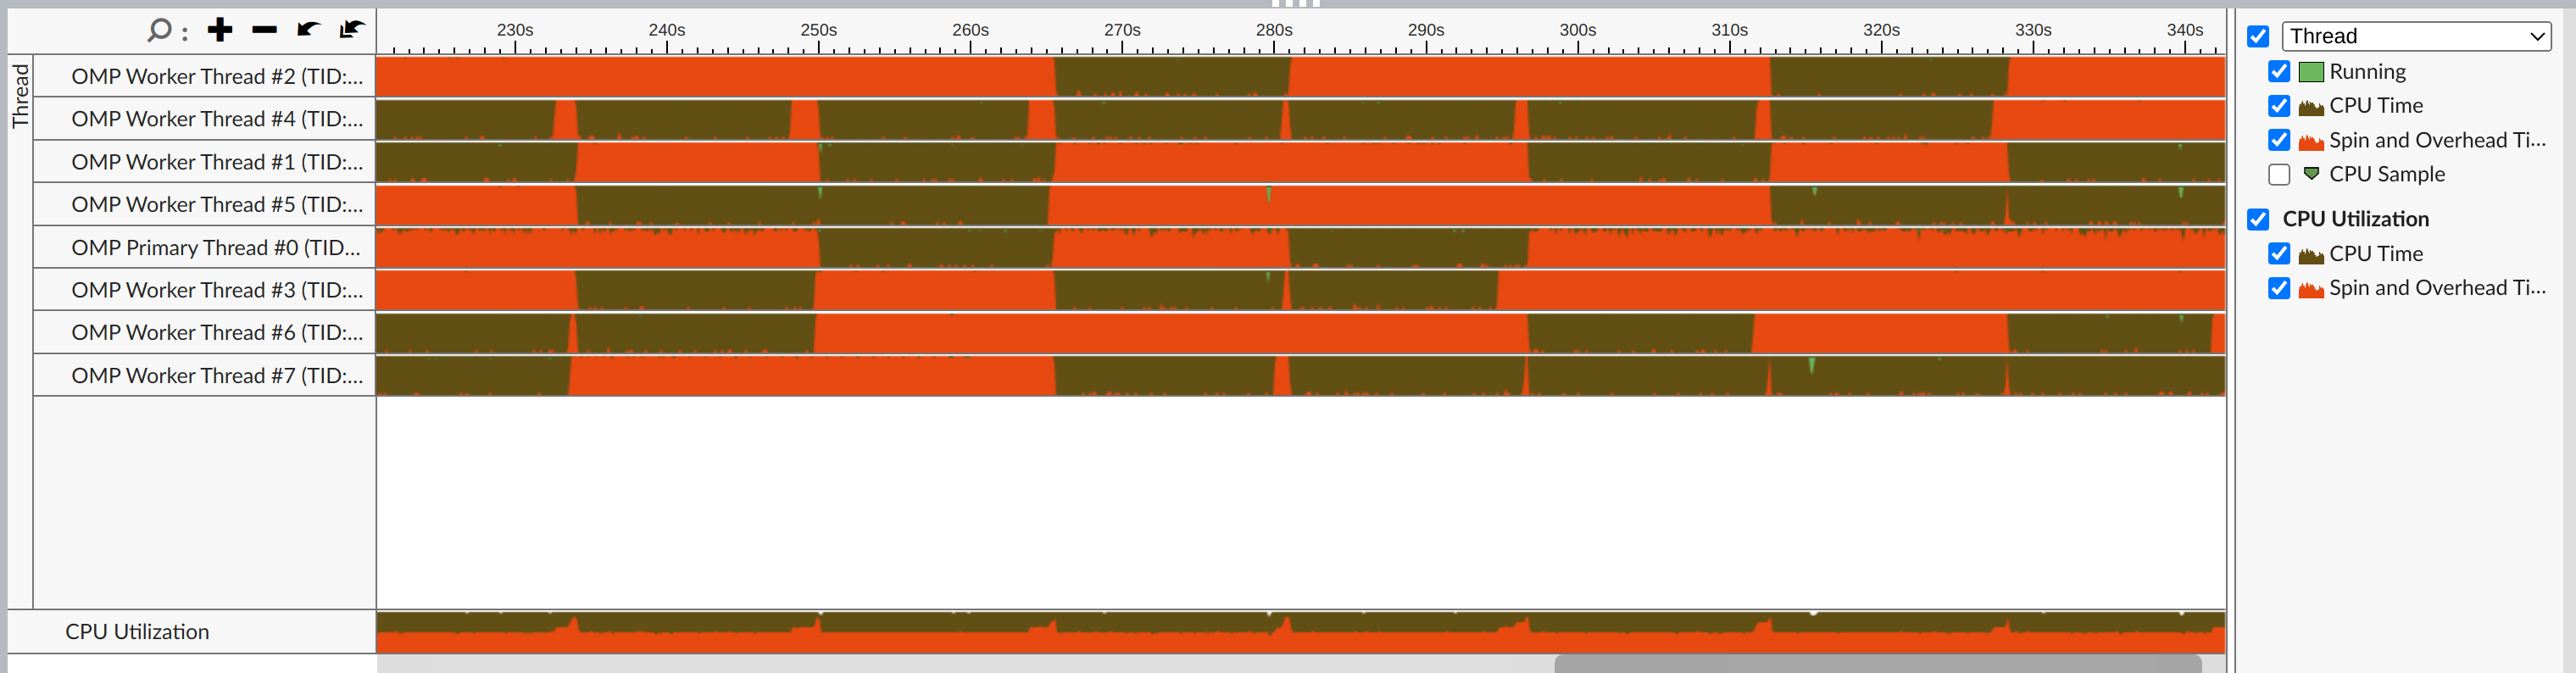
\includegraphics[width=0.7\textwidth]{node-level/vtune-imbalance-00.png}
 \end{center}
 
 \noindent
 The idle threads here don't really idle: They continue to run even if they have nothing to do, but spin all the time, i.e.~wait busily for new work to drop in. 
 We can dig deeper with the \emph{HPC Performance Characterization} analysis, where we see imbalances broken down over individual functions or loops, respectively.
 The mode is particularly useful for loop-/data-parallelism.
 For code that relies a lot on tasks, it is not straightforward to localise imbalances, and we might have to do some manual analysis work.

 \begin{center}
   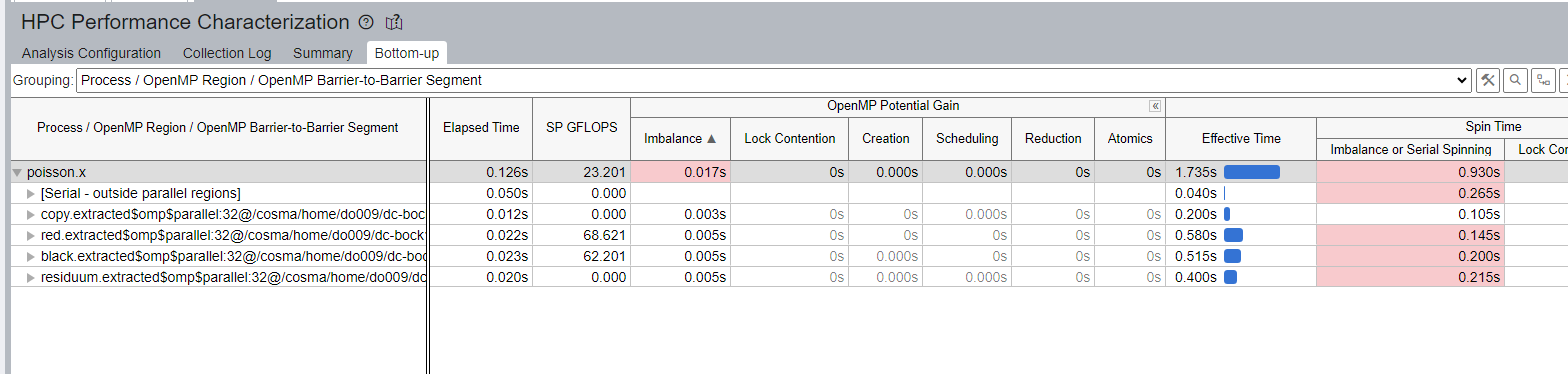
\includegraphics[width=0.7\textwidth]{node-level/vtune-imbalance-01.png}
 \end{center}
\end{instructions}


\subsection{Evaluation}


\begin{enumerate}[noitemsep]
  \item[$\boxtimes$] The work is perfectly balanced, but the performance remains poor.
    \begin{itemize}[noitemsep]
      \item[$\Rightarrow $] Study the average task size and investigate whether these tasks can be split up further (Section~\ref{xxxx}).
    \end{itemize}
  \item[$\boxtimes$] The work is not perfectly balanced.
    \begin{itemize}[noitemsep]
      \item[$\Rightarrow $] 
Natural performance optimisations are switching to smaller grain sizes (iteration space chunks) or to enable dynamic scheduling if the individual chunks have largely varying runtimes.
However, these are already code tweaks, i.e.~beyond the scope of this handbook.
    \end{itemize}
\end{enumerate}




\paragraph*{How it works}

\begin{itemize}[noitemsep]
  \item[$\boxplus$] Track how long the cores actually compute and compare it to the time where they do not deliver science.
  \item[$\boxplus$] If there are severe imbalances, continue to work through hypotheses to find out where the imbalances come from and reduce the granularity such that there are enough pieces of work.
\end{itemize}


\paragraph*{How it does not work}

\begin{itemize}[noitemsep]
  \item[$\boxminus$] Stop the analysis once the work is perfectly balanced. Performance might still suffer from overheads.
\end{itemize}

